% 编码格式: "TeX:UTF-8"
% tex编译链 = xelatex
% Created by tinoryj on 2017/2/27.
% Copyright © 2017年 tinoryj. All rights reserved.
% 模版支持三级标题,如果需要插入第四级
% lipsum[1] 为模版文字,使用时自行删除
% 基于2011版格式要求设计,针对现行电子版不要求前两页信息进行设计。

%\documentclass[bwprint]{cumcmthesis}
\documentclass[withoutpreface,bwprint]{cumcmthesis} %去掉封面与编号页

\title{模版}
\tihao{A/B}
\baominghao{201723003002}
\schoolname{电子科技大学}
\membera{卫佳杰}
\memberb{谢沁余}
\memberc{任彦璟}
\supervisor{覃思义}
\yearinput{2017}
\monthinput{09}
\dayinput{17}

\begin{document}
 \maketitle
 
 \begin{abstract}
 %摘要正文
 \lipsum[1]
 
\keywords{关键字1}

\end{abstract}





\section{模型的假设}
\begin{itemize}
	\item ...
\end{itemize}
\section{符号说明}
\begin{tabular}{cc}
 \hline
 \makebox[0.4\textwidth][c]{符号}	&  \makebox[0.5\textwidth][c]{意义} \\ \hline
 ..	    &  .. \\ \hline
\end{tabular}
\section{问题分析}
\subsection{问题一分析}
\lipsum[1]
\subsection{问题二分析}
\lipsum[1]
\subsection{问题三分析}
\lipsum[1]

\begin{figure}[!h]
\centering
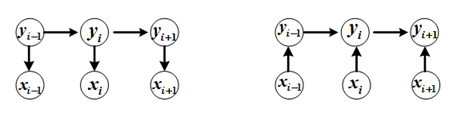
\includegraphics[width=\textwidth]{1.png}
\caption{问题三流程图}
\end{figure}
\begin{thebibliography}{9}
 \bibitem{bib:one} ....
 \bibitem{bib:two} ....
\end{thebibliography}
\appendix
\section{程序}
cpp\textcolor[rgb]{0.98,0.00,0.00}{\textbf{Input C++ source:}}
% 代码插入,请将代码文件放入code文件夹,支持语言的语法高亮。支持语言:C,C++,Java,Matlab,Mathematica,python,R,可在cls文件中自行添加。
\lstinputlisting[language=C++]{./code/a.cpp}


\end{document} 